\section{Versuchsdurchführung}




\subsection*{Charakterisierung des Aufbaus}
Vor Durchführung der Kernspinresonanz-Messung werden
zwei Messreihen zur Charakterisierung des Aufbaus durchgeführt:\\
Mit der Hall-Sonde wird der gesamte Bereich der Probenhalterung in senkrechter
Richtung abgefahren und in 5\,mm-Schritten die Stärke des Magnetfelds bestimmt.\\
Dann wird bei fester Position der Hall-Sonde (20\,mm unter der Oberkante der Öffnung) die Abhängigkeit
der Magnetfeldstärke vom Spulenstrom untersucht,
um später schnell gewünschte Feldstärken einstellen zu können.

\subsection*{Messung der Kernspinresonanz an Wasser, Teflon und Glykol}
Die Messung der Kernspinresonanz an Wasser wird für feste Frequenzen des HF-Wech\-sel\-fel\-des
(zwischen 16\,MHz und 19\,MHz in 0.5\,MHz-Schritten)
durchgeführt und für jede Frequenz der Strom für das statische Magnetfeld am Netzteil so eingestellt,
dass am Oszilloskop die Minima der Absorption gleich weit voneinander entfernt sind (\autoref{img:oszi}).
Für jeden eingestellten Strom wird durch eine Messung mit der Hall-Sonde die Magnetfeldstärke gemessen.\\
Danach wird mit dem selben Messprinzip je ein Messpunkt bei 17.5\,MHz für Teflon und für Glykol aufgenommen.

\begin{figure}[H]
\begin{center}
  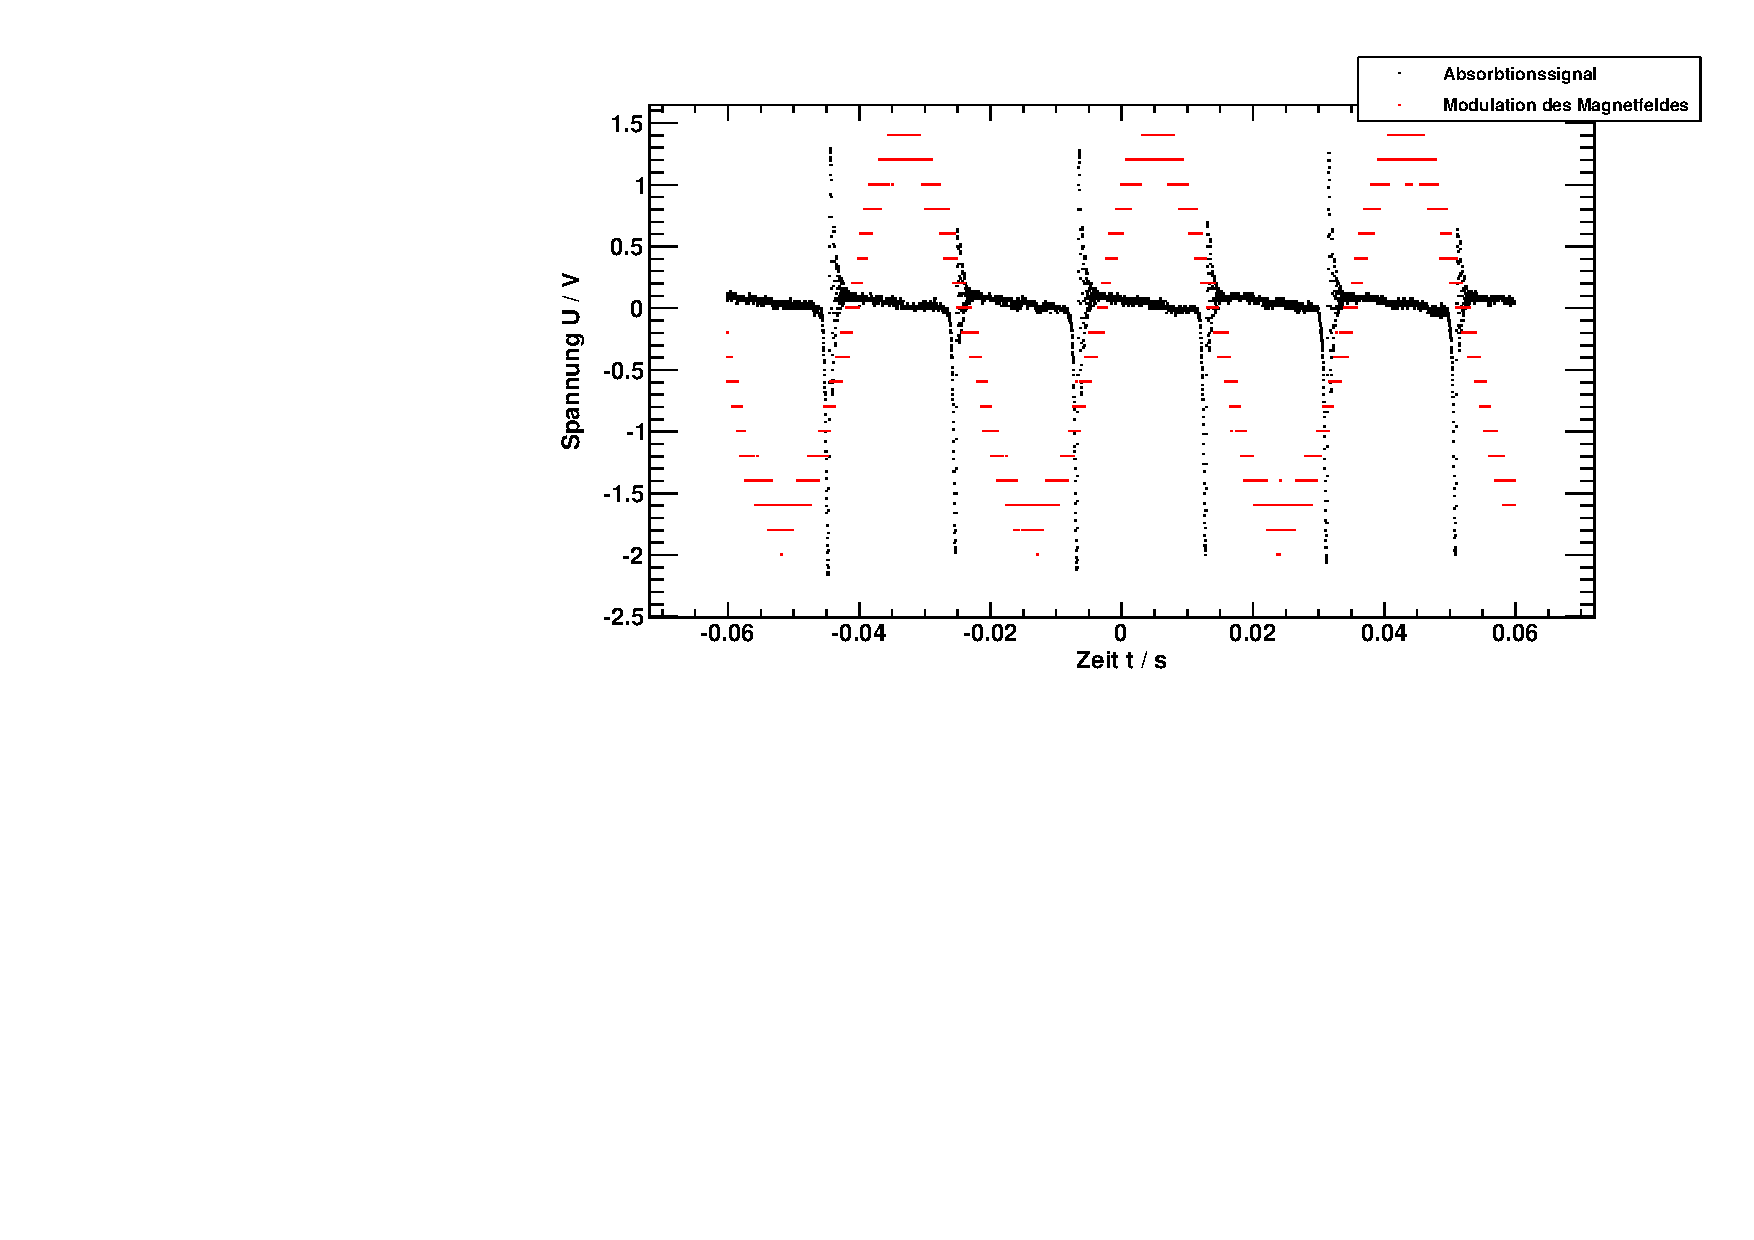
\includegraphics[width=\textwidth]{../img/graph_02.pdf}
  \caption{Geeignete Einstellung des statischen Magnetfeldes, so dass die Resonanz zwei mal pro Periode getroffen wird. 
  (Hier mit Wasserstoff, $\nu=16.0220$\,MHz, $B=372$\,mT)}
  \label{img:oszi}
\end{center}
\end{figure}
